\chapter{Функциональное тестирование}

Функциональные тесты основываются на функциях, выполняемых системой. Как правило, эти функции описываются в требованиях, функциональных спецификациях или в виде случаев использования системы (use cases).

\section{Use Cases}

\textbf{Use Case} — это сценарная техника описания взаимодействия. С помощью Use Case может быть описано и пользовательское требование, и требование к взаимодействию систем, и описание взаимодействия людей и компаний в реальной жизни. В общем случае, с помощью Use Case может описываться взаимодействие двух или большего количества участников, имеющее конкретную цель. В разработке ПО эту технику часто применяют для проектирования и описания взаимодействия пользователя и системы, поэтому название Use Case часто воспринимает как синоним требования человека-пользователя к решению определенной задачи в системе.


Примеры Use Case для тестируемого приложения:
\begin{enumerate}
	\item авторизация пользователя с вводом текущего города
	\item добавление пользователем исполнителей в личный список подписок
	\item удаление пользователем исполнителей из своего списка
	\item вывод подписки в виде списка
	\item вывод ближайших концертов исполнителей из подписок в городе пользователя
\end{enumerate}

\subsection{Основные действия пользователя }

\begin{enumerate}
	\item пользователь авторизует себя отправляя сообщение /start боту
	\item пользователь указывает город через запрос /city 'город пользователя'. Не выполнив данный шаг, бот будет отказываться выполнять любые действия.
	\item пользователь начинает заполнять свой лист подписок с помощью /add 'имя исполнителя'
	\item пользователь выводит подписки с помощью команды /list
	\item если пользователь хочет убрать исполнителя из подписок, то он вводит /remove 'имя исполнителя'
	\item если же пользователь хочет полностью очистить лист подписок, то он вводит /clear 
\end{enumerate}
При всех запросах, указанных выше, сервер производит действия с базой данных для изменения/добавления информации. 

\subsection{Тестирование основных действий}
Для проверки обработки основных запросов было проведено функциональное тестирование.
\begin{table} 
	\caption{Функциональное тестирование}
	\begin{center}
		\begin{tabular}{|l|p{10cm}|}
			\hline
			\multicolumn{2}{|c|}{Обновление города пользователя} \\
			\hline
			Запрос & /city Town \\
			Ожидаемый результат &  "Ваш город обновлен, теперь вы находитесь в городе Town" \\
			\hline
			\multicolumn{2}{|c|}{Добавление пользователя(начальная авторизация)} \\
			\hline
			Запрос & /city Town \\
			Ожидаемый результат &  "Поздравляем с регистрацией, ваш город Town" \\
			\hline
			\multicolumn{2}{|c|}{Добавление пользователя с существующим userid} \\
			\hline
			Запрос & /city 'любой город' \\
			Ожидаемый результат &  Ничего \\
			Примечание & данный тест необходим для сервера, т.к. в данном случае на сервер будет отправлена информация о возникшей ошибке. Пользователь же в данном случае никак не пострадает, т.к. если такой userid уже существует, то база данных никак не обновится. Информация серверу посылается для отладки, если в базе данных возникнут конфликты при добавлении пользователя с одинаковым первичным ключом. \\
			\hline
			\multicolumn{2}{|c|}{Вывод списка подписок состоящей из 'group1'} \\
			\hline
			Запрос & /list \\
			Ожидаемый результат &  "1)group1 "\\
			\hline
			\multicolumn{2}{|c|}{Удаление 3-ей группы из подписки с 3 группами} \\
			\hline
			Запрос & /remove group3 \\
			Ожидаемый результат &  "Исполнитель group3 удален из подписок" \\
			\hline
			\multicolumn{2}{|c|}{Удаление группы отсутствующей в подписках} \\
			\hline
			Запрос & /remove group22\\
			Ожидаемый результат &  Список подписок без изменений \\
			\hline

			

		\end{tabular}
	\end{center}
\end{table} 


\begin{table} 
	\begin{center}
		\begin{tabular}{|l|p{10cm}|}
			\hline
			\multicolumn{2}{|c|}{Вывод пустого списка подписок} \\
			\hline
			Запрос & /list \\
			Ожидаемый результат &  "Добавьте группу с помощью команды \"/add <Группа>\"." \\
			\hline
			\multicolumn{2}{|c|}{Попытка вывести список подписок, не указав город} \\
			\hline
			Запрос & /list \\
			Ожидаемый результат &  "Пользователь с таким id не найден. Добавьте город с помощью \"/city" \\
			\hline
			\multicolumn{2}{|c|}{Полная очистка подписок} \\
			\hline
			Запрос & /clear \\
			Ожидаемый результат &  "Ваш список подписок очищен"\\
			\hline
			\multicolumn{2}{|c|}{Вывод списка подписок из 2-ух групп после удаление второй} \\
			\hline
			Запрос & /remove group2 \\
			Ожидаемый результат &  "1) group1"\\
			\hline
			\multicolumn{2}{|c|}{Вывод списка подписок из 3-ух групп после удаление второй} \\
			\hline
			Запрос & /remove group2 \\
			Ожидаемый результат &  "1) group1 2)group3"\\
			\hline
			\multicolumn{2}{|c|}{Вывод ближайших концертов(при отсутствии концертов в городе пользователя)} \\
			\hline
			Запрос & /show\\
			Ожидаемый результат &  "Не найдено ни одного концерта в вашем городе у исполнителей из вашего списка подписок, однако они выступают в России "\\
			\hline
			\multicolumn{2}{|c|}{Вывод ближайших концертов(при наличии концерта в городе пользователя)} \\
			\hline
			Запрос & /show\\
			Ожидаемый результат & "Инфо о концерте группы {0} Название: {1} Место: {2} Время: {3} Ссылка на источник: {4} "\\
			\hline
			\multicolumn{2}{|c|}{Вывод ближайших концертов(при отсутствии концертов в принципе )} \\
			\hline
			Запрос & /show\\
			Ожидаемый результат & "Не найдено ни одного концерта в вашем городе у исполнителей из вашего списка подписок "\\
			\hline
			
			
		\end{tabular}
	\end{center}
\end{table} 
\newpage
\section{Покрытие}
\begin{figure} [h]
	\centering
	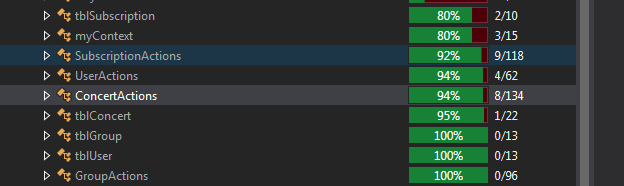
\includegraphics[scale=1]{CoverFunctional.PNG}
	\caption{Покрытие после модульных,интеграционных, функциональных тестов}
	\label{image:cover-functional}
\end{figure}
Как можно заметить было достигнуто практически полное покрытие основных классов.